
\begin{multicols}{2}
A l'aide de la figure ci-contre, on
  cherche à déterminer la longueur $AM$ du point $M$ visible de $A$ et
  $B$. Les données connues sont indiquées sur la figure : $AM=a$;
  $\widehat{MAB}=\alpha$ et $\widehat{ABM}=\beta$. Dans le triangle
  $ABM$, $H$ est le pied de la hauteur issue de $A$.
  \begin{enumerate}
    \item On appelle $\gamma$ l'angle $\widehat{AMB}$. Exprime
      $\gamma$ en fonction de $\alpha$ et $\beta$.
    \item 
      \begin{enumerate}
      \item Exprime la longueur $AH$ en fonction de $AB$ et $\beta$.
      \item Exprime la longueur $AH$ en fonction de $AM$ et $\gamma$.
      \end{enumerate}
    \item Déduis-en la formule qui permet de calculer $AM$ en fonction
      de $AB$, $\alpha$ et $\beta$.
  \end{enumerate}
 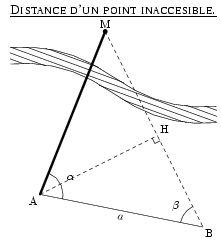
\includegraphics[scale=1]{TR-215.png}  
  \end{multicols}